\documentclass{article}[18pt]
\usepackage{../../../../../format}
\lhead{Computer Systems}
\usepackage{karnaugh-map}

\begin{document}
\begin{center}
\underline{\huge Karnaugh Maps}
\end{center}
\section{Simplifying Boolean Expressions}
Key to simplifying is spotting terms of the form $PA+P\overline{A}$ (Since this is P)\\
\\
\textbf{Karnaugh Maps} are a graphical way of representing equations to make spotting these terms easier
\begin{center}
	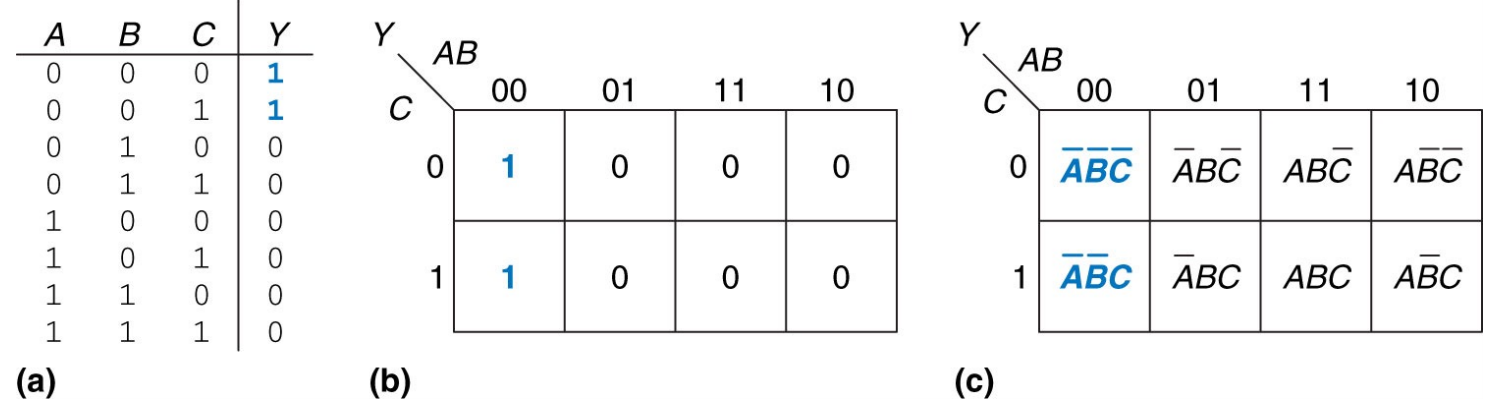
\includegraphics[scale=0.5]{karnaughex}
\end{center}
Each cell represents a minterm, and has a 0 or 1 depending on the value of Y corresponding to that minterm. SoP form is given by the 1s\\
\\
The order of minterms is such that each cell differs in \textbf{the negation of exactly one variable} from its neighbours (including wrap around) - this is why they are not in numerical order\\
\\
\\
Terms of the form $PA+P\overline{A}$ are neighbouring 1s in the K-map\\
\begin{karnaugh-map}*[4][2][1][AB][C]
	\minterms{0,4}
	\autoterms[0]
	\implicant{0}{4}
\end{karnaugh-map}\\
Rather than filling out the full SoP by taking every 1 as a term, we circle the neighbouring 1s, and use a single reduced implicant for both 1s in the circle:
\textbf{Full SoP reduced}:
$$Y=\overline{ABC}+\overline{AB}C$$
$$Y=\overline{AB}$$
\section{Karnaugh Maps}
\begin{enumerate}
	\item Create a map so that neighbouring terms differ in the negation of one variable (including wrap around)
	\item Circle all rectangular blocks of ones in the map using as few circles as possible. But make the circles as big as possible
	\item Each circle must be a power of 2 in each dimension (i.e. 1,2,4)
	\item Read off the implicants that were circled
\end{enumerate}
If a boolean expression is minimal then it is the sum of \textbf{prime implicants}: implicants that cannot be combined with each other\\
\\
Each circle represents an implicant. Largest possible circles represent prime implicants
\section{Example}
\begin{karnaugh-map}[4][2][1][AB][C]
	\minterms{0,2,3,4,6}
	\autoterms[0]
	\implicantedge{0}{4}{2}{6}
	\implicant{3}{2}
\end{karnaugh-map}\\
Red - $\overline{B}$\\
Green - $A\overline{C}$\\
\\
\textbf{SoP}:
$$Y=\overline{ABC}+A\overline{B}C+AB\overline{C}+\overline{AB}C+A\overline{B}C$$
\textbf{Using the K-map}
\begin{itemize}
	\item Circle 1s
	\item Notice that we can wrap around
	\item We cannot do a 3 by 1 rectangle
	\item Can still cover the 1s with only 2 rectangles
\end{itemize}
So the SoP can then be simplified down to
$$Y=\overline{B}+A\overline{C}$$
\section{Example}
\begin{center}
	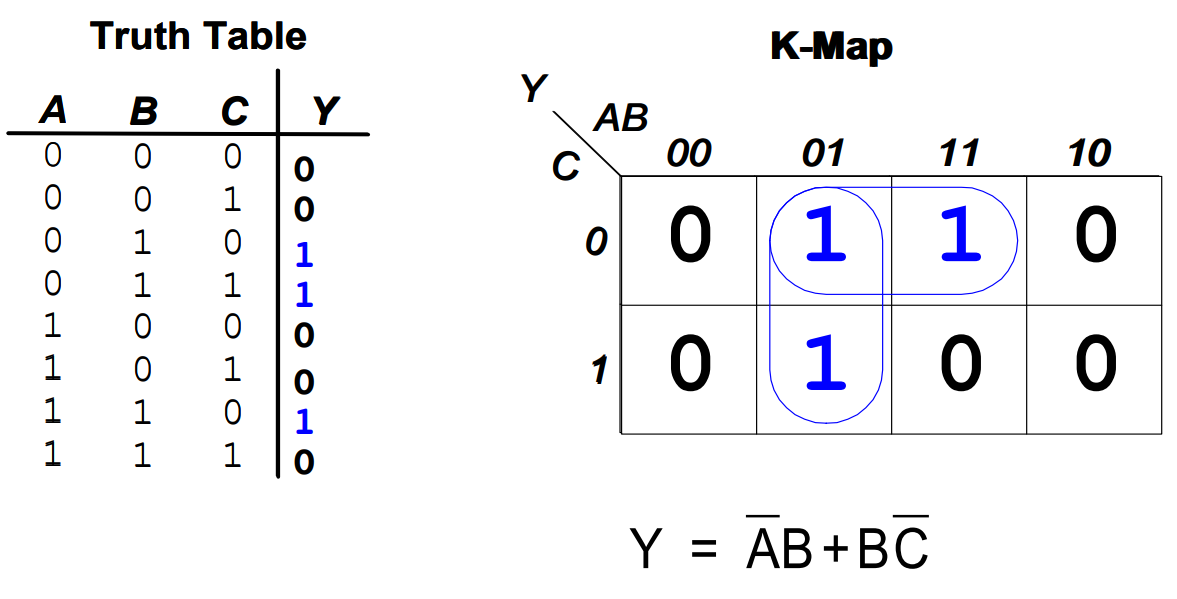
\includegraphics[scale=0.4]{karnaughex1}
\end{center}
\section{4026 decade counter and 7-segment display driver}
\begin{center}
	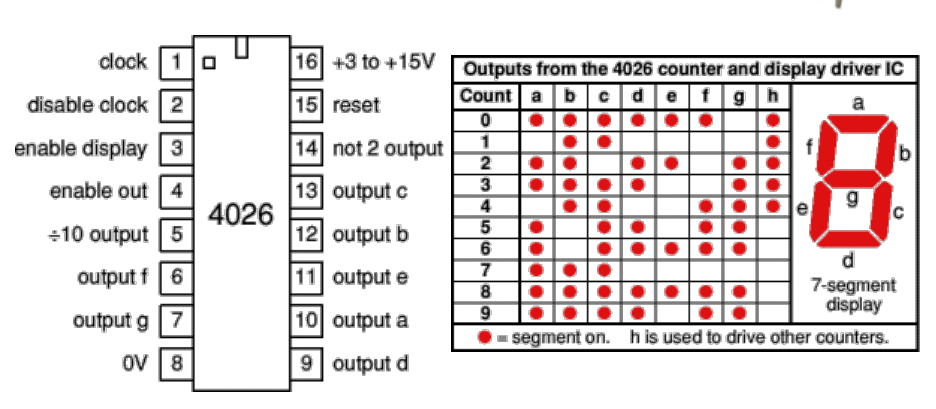
\includegraphics[scale=0.5]{4026decade}
\end{center}
\subsection{7-Segment Display Driver}
\begin{center}
	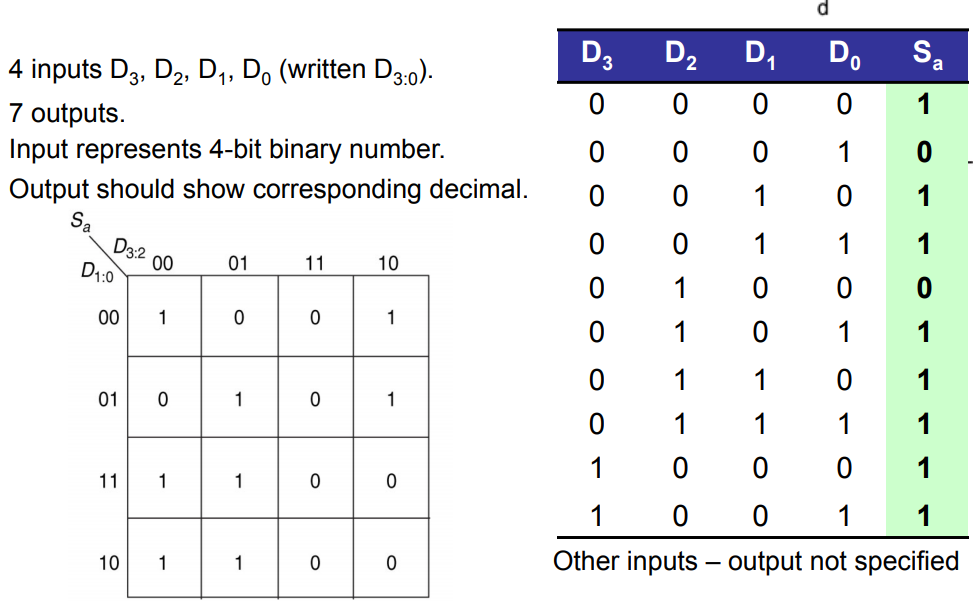
\includegraphics[scale=0.5]{7seg}
\end{center}
\subsubsection{Karnaugh Map}
\begin{center}
	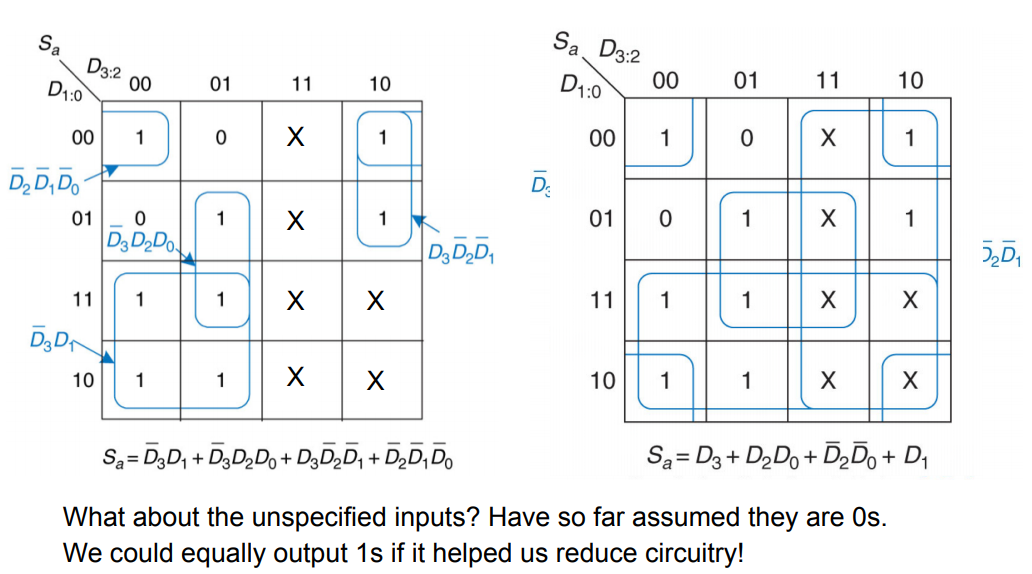
\includegraphics[scale=0.5]{7se_Karnaugh1}
\end{center}
\begin{itemize}
	\item If inputs are unspecified, then use an X rather than a zero, as it may be a 1
	\item From the SoP it is then simple to produce a circuit by just satisfying the requirements
\end{itemize}


\begin{center}
	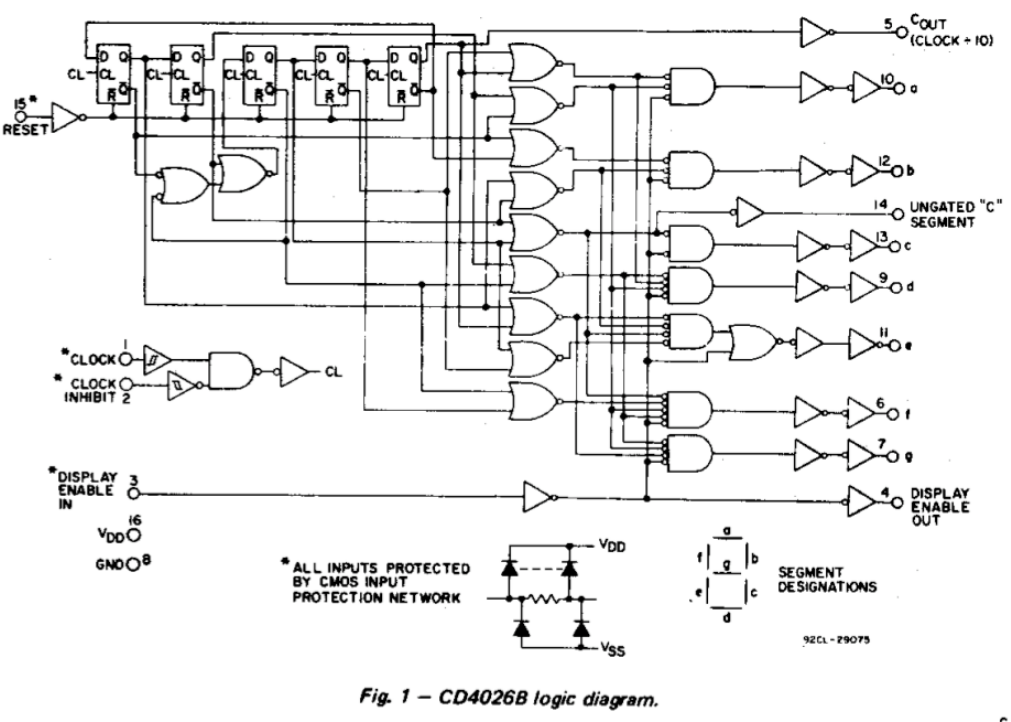
\includegraphics[scale=0.7]{circuit1}
\end{center}
\begin{center}
	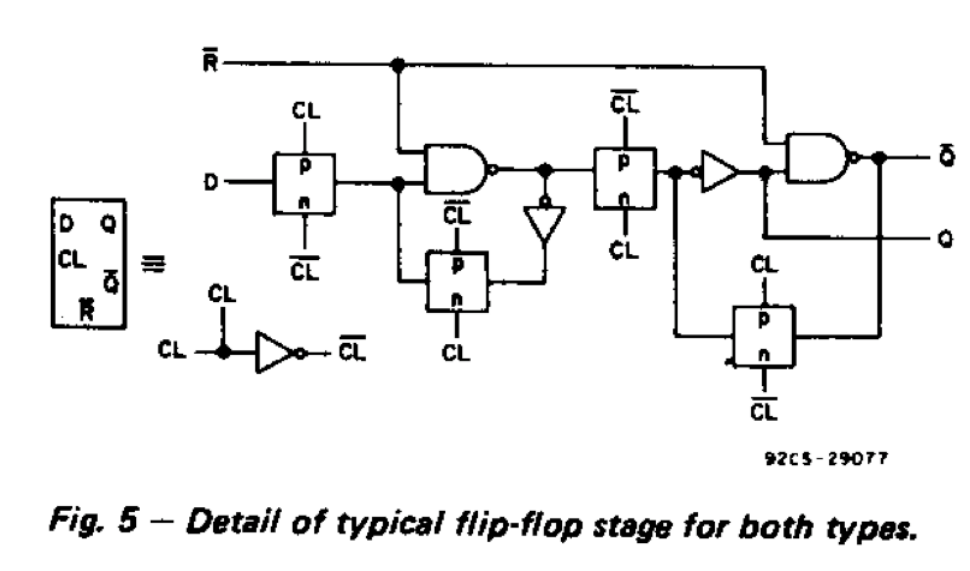
\includegraphics[scale=0.5]{circuit2}
\end{center}
\subsection{Description}
The count advances as the clock input becomes high (on the rising-edge). The outputs a-g go
high to light the appropriate segments of a common-cathode 7-segment display as the count
advances. The maximum output current is about 1mA with a 4.5V supply and 4mA with a 9V
supply. This is sufficient to directly drive many 7-segment LED displays. The table below
shows the segment sequence in detail.\\
\\
The reset input should be low (0V) for normal operation (counting 0-9). When high it resets the count to zero.\\
\\
The disable clock input should be low (0V) for normal operation. When high it disables counting
so that clock pulses are ignored and the count is kept constant.\\
\\
The enable display input should be high (+Vs) for normal operation. When low it makes outputs
a-g low, giving a blank display. The enable out follows this input but with a brief delay.\\
\\
The $\div$10 output (h in table) is high for counts 0-4 and low for 5-9, so it provides an output at 1/10
of the clock frequency. It can be used to drive the clock input of another 4026 to provide
multi-digit counting.\\
\\
The not 2 output is high unless the count is 2 when it goes low.







\end{document}